% !TEX root =  main.tex
\section{Introduction}
\subsection{Motivation}

Building systems that can understand and reason with information present in texts is a central pursuit in the AI vision. Extracting from texts is a challenging task in itself and requires access to open-domain knowledge. It is no surprise that these articles written for human consumption assume background knowledge and an inference capability that reads between lines. For example, consider extracting information from the following news snippet:

\begin{verbatim}
        Somalia's al-Shabab militant group has confirmed the death 
        of its leader in a U.S. airstrike and named his successor. 
        The al-Qaida linked militants announced the selection of 
        Abu Ubeid Ahmed Omar to replace Abdi Godane. 
\end{verbatim}
Reading these two sentences, we can easily determine the important information: {\em Abdi Godane} was the leader of {\em al-Shabab}, a {\em terrorist group}, {\em Abu Ubeid Ahmed Omar} is the successor of {\em Abdi Godane}, and {\em Abdi Godane} was killed by a {\em U.S.} airstrike.  Note we also make inferences along the way. None of this information is explicitly mentioned in the sentences. Automatic extraction systems on the other hand, need to be told what information to extract -- e.g, the one who gets replaced, the successor, the position being filled, the employing organization etc. This kind of declarative knowledge also provides constraints that can help resolve referential ambiguities and extract implicit relations. %Such knowledge can also provide effective guidance for producing effective summaries. 

Existing state-of-the-art information systems do not have access to this kind of open-domain knowledge.
For example, Open information extraction (Open IE) systems extract {\em every} possible binary relation explicitly stated in text because they do not have any notion of salience. Moreover, most events and scenarios involve multiple participants with specific roles that are not effectively represented by binary relations. 

Template-driven extraction aims to address these issues by pre-specifying an extraction template or a schema for each event type (e.g., arrest, arson, bombing). Schemas describe an event type in terms of the actors and the roles they play within the event. An arrest schema, for example, will include an arresting agent who arrests and charges a suspect, a lawyer and a judge who rules on the case, as its key participants. 

Until recently the cost of manual authoring had limited template-based information extraction to a handful of domains. 
Prior attempts at automatically generating event schemas suffer from coherence issues -- mixing distinct events (e.g, fire spreading vs. disease spreading)~\cite{chambers-acl09}. The lack of event schemas covering a broad range of domains is a fundamental challenge in scaling event extraction. 

\subsection{Proposal}
\begin{figure}[thb]
	\begin{center}
	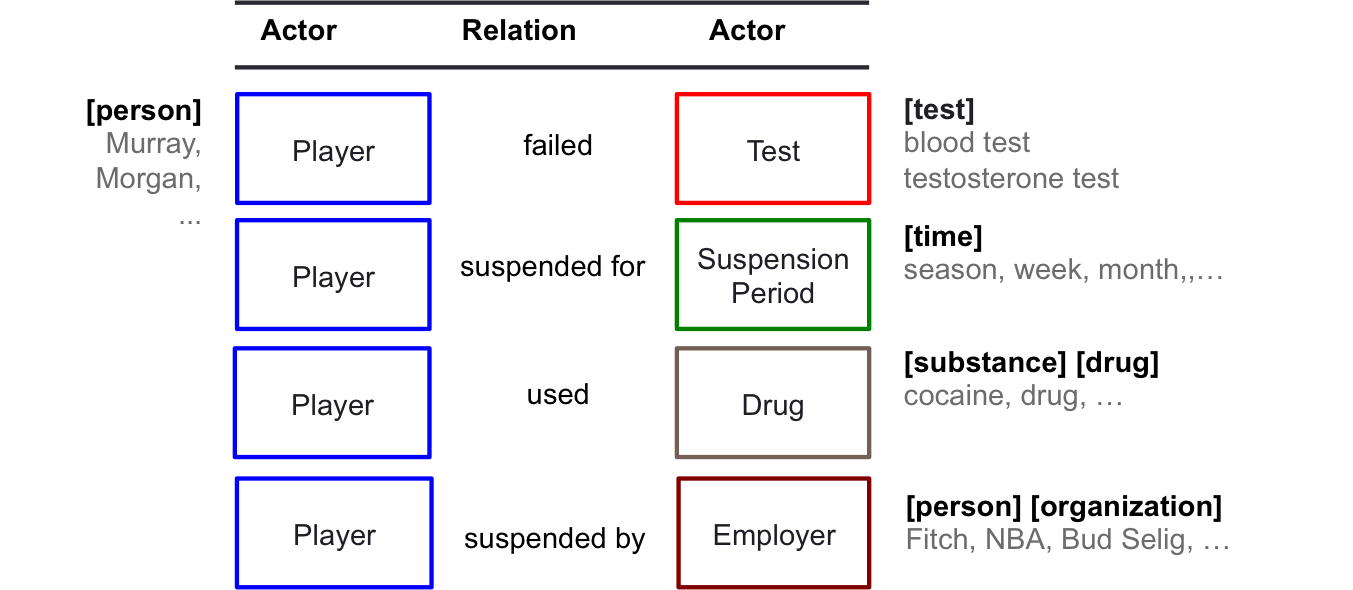
\includegraphics[width=5.7in,height=2.5in]{figures/drug-schema} 	
	\caption{\label{fig:drug-schema} {Drug Suspension Schema, which specifies the participants (actors) involved and their roles. The square boxes represent the participants. The semantic types of the participants are shown by their side along with some example instances for each participant.}}
	\end{center}
\end{figure}
In this work, I propose to tackle the main challenges in schema-based event extraction. I propose to investigate automatic methods for high-quality schemas and will produce a large scale curated collection to promote further research in this area. In particular, I will target generation of schemas that specify the participants (actors) and their roles via generalized relations with semantically typed arguments. Figure~\ref{fig:drug-schema} shows an example that represents information about a scenario where a player gets suspended for taking a drug. The key participants include the player, the drug used, the test they failed and the punishment. The relations indicate the roles the participants play.  

To this end, this proposed work will include the following activities:
\begin{enumerate}[nolistsep,noitemsep]
\item Develop representations and algorithms for automatically generating open-domain event schemas. I will investigate corpus-based techniques that exploit relation co-occurrence to identify generalized relations that belong in a schema. This involves handling significant research challenges in a) generating effective representations while also addressing the resulting sparsity issues, and b) building effective graph-based algorithms that can identify clusters of co-mentioned relations. 
\item Develop techniques to build extractors using these event schemas. The main scope of this activity is to keep the schema generation effort grounded in this end task and to demonstrate the feasibility of open-domain event extraction, 
\item Create a large scale curated collection of automatically generated open-domain event schemas (~10K) and an event extraction dataset.
\end{enumerate}

\subsection{Contributions}
The proposal builds upon the initial results and key findings in our prior work for automatically generating coherent event schemas~\cite{balasubramanian-akbc12,balasubramanian2013generating}. Exploiting recent advances in relation extraction technology, as well as large scale resources (e.g., NELL, Freebase), I will target automatic generation of high quality event schemas and release large scale datasets to further event extraction research. 

Successful completion of the proposed activities will make the following technical contributions:
\begin{itemize}[noitemsep,nolistsep]
\item An effective representation for events that reduces ambiguity and techniques to address sparsity.
\item Graph-based approaches that use graphical properties to address topic-drift in order to produce high-quality schemas.
\item Effective bootstrapping techniques for building extractors for schema elements.
\item  A large scale collection of manually curated open-domain schemas and large scale evaluation data set for event extraction that covers a wide range of domains.
\end{itemize}
\newpage


\eat{
In this work, we target extraction of rich event schemas that describe events using a range of information as shown in the table below.
\begin{table}[htdp]
\caption{default}
\begin{center}
\begin{tabular}{|p{4cm}|p{12cm}|}
\hline
Entities & Extractors\\
& Researcher, Organization, Subject, Problem, Conclusion, Publication, Date, Location \\
\hline
Sub-events &  \\
& R: Researcher study Problem (X)\\
& R find found/discovered/uncovered/stumbled/ Conclusion (Y) \\
& R published Results/Conclusions in [Journal/Book/Conference] \\
& R supports/refutes \\
& \\
\hline
Background-relations & \\
& R: Researcher, employed by, O:[Organization] \\
& study: Research, funded by, O:[Organization] \\
\hline
Entity Extractors & \\
& X:[Person] studies Y: [Problem] $\rightarrow$ X: [Researcher] \\
& X is studied by Y: [Person] $\rightarrow$ X: [Subject]\\
& X: [Researcher] concludes Y $\rightarrow$ Y: [Conclusion]\\
\hline
Relation Extractors & \\
	& study -- studied, investigated, explored, asked\\
	& find -- discovered, uncovered, stumbled \\			
\hline
Dependencies (Rel-grams) & \\
& R found Y, Conclusion(Y) $\rightarrow$ R publishes Y \\
& R found Y, Conclusion(Y) $\rightarrow$ R studied X \\	
\hline
Related Scripts & \\
& investigate, publish \\
\hline
\end{tabular}
\end{center}
\label{default}
\end{table}%

}


%To effectively address these issues, extraction systems need background knowledge that provide models or expectations for the information they need to extract. For example models of salient aspects of certain types of entities (e.g., actors {\em act in} movies, actors {\em win} awards) can help extract and organize information about people. Similarly, rich descriptions of events or scenarios, processes and their interactions can help in extracting and understanding information about events from texts. Scalable methods for acquiring such background knowledge is essential for building broad coverage extractors.

%These open-domain event schemas are but a starting point for aggregating and organizing background knowledge about events that can be leveraged during extraction. The main goal of this project is to build open-domain script like knowledge about events. 

%Script-like knowledge serve as general purpose description of events or scenarios. In addition to the key actors, their actions, we will build scripts that include causal, temporal and dependency relationships between the different actions. During extraction this richer representation will enable us to infer more than what is explicitly mentioned in the text. 

%Schemas provide a high precision model of scenarios which can be expanded to associated extractors -- i.e., patterns that can be used to extract from new texts. Resolving entity and event co-references. Third, scripts must include causal and temporal ordering of the actions in a scenario. 

%\subsection{Research Challenges}
%\subsection{Contributions}
